\section{Auswertung}
\label{sec:Auswertung}

\subsection{Reflektion}
  Für die Reflektion wurden für die Einfallswinkel $\alpha_1$ die in Tabelle \ref{tab:angle} dargestellten Ausfallswinkel (in Grad)
  gemessen.
  \begin{table}[H]
    \centering
    \caption{Werte der Reflektion}
    \begin{tabular}{c c}
      \toprule
      $\alpha_1$ & $\alpha_2$\\
      \midrule
        20 & 20.5 \\
        30 & 31   \\
        40 & 41   \\
        45 & 46   \\
        50.5 & 51 \\
        60 & 60.5 \\
        70 & 71   \\
      \bottomrule
    \end{tabular}
    \label{tab:angle}
  \end{table}
  \noindent Diese wurden in der Abbildung \ref{fig:plot2} dargestellt und ihre Steigung $m=1.001 \pm 0.007$
  mittels linearer Regression bestimmt.
  \begin{figure}[H]
    \centering
    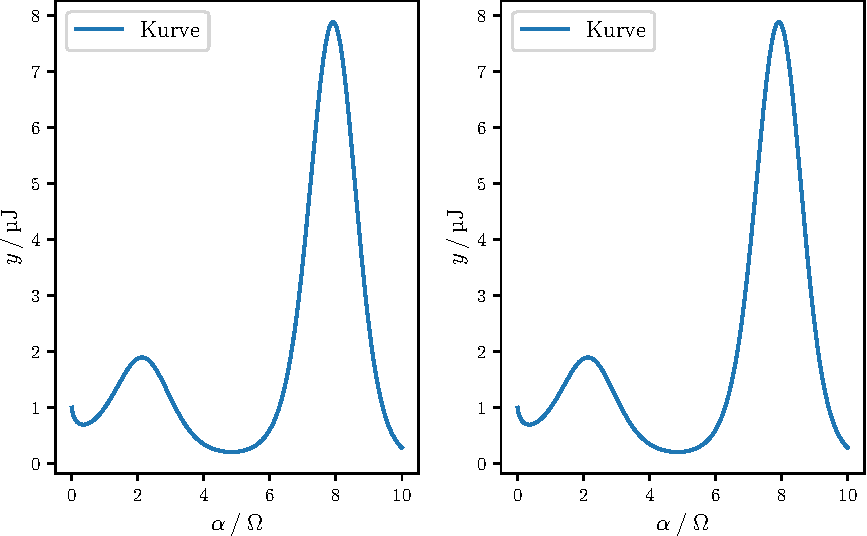
\includegraphics{plot.pdf}
    \caption{Messwerte der Reflektion}
    \label{fig:plot2}
  \end{figure}

\subsection{Transmission}
  Zu den Einfallswinkeln $\alpha$ ergab der zweite Versuch die in Tabelle \ref{tab:trans} gezeigten 
  Brechungswinkel $\beta$.
  \begin{table}[H]
    \centering
    \caption{Werte der Transmission}
    \begin{tabular}{c c c}
      \toprule
      $\alpha$ & $\beta$&$n$\\
      \midrule
        10 & 7.25& 1.38 \\
        20 & 13.5& 1.48 \\
        30 & 20  & 1.49 \\
        40 & 26  & 1.52 \\
        50 & 31.5& 1.56 \\
        60 & 36  & 1.61  \\
        70 & 39.5& 1.69 \\
      \bottomrule
    \end{tabular}
    \label{tab:trans}
  \end{table}
  \noindent Daraus lassen sich anhand der Formel $n = \dfrac{\sin{\alpha}}{sin{\beta}}$ die
  Werte in für den Brechungsindex n berechnen.
  \noindent Mittels Numpy wurde daraus der Mittelwert $n=1.53\pm 0.04$ beestimmt. Anhand 
  dieses Wertes wurde die Lichtgeschwindigkeit in dem Glas zu $c_G=\dfrac{c}{n}= (1.95\pm 0.05)
  \cdot 10^{8}$ m/s berechnet.

\subsection{Strahlversatz}
  Für diesen Abschnitt wurden dieselben Werte verwendet, die bereits für den Abschnitt 
  Transmission verwendet wurden.
  Mit der in der Theorie hergeleiteten Formel 
  \begin{equation*}
    s= d\dfrac{\sin{\alpha - \beta}}{cos{\beta}} 
  \end{equation*}
  wird nun der Strahversatz berechnet. Dabei wird zunächst mit den realen Beta-Werten und dann
  mit idealisierten, die durch $\beta=\arcsin{\dfrac{\sin{\alpha}}{n}}$ wurden. Dabei ergeben 
  sich für $\beta$ die in Tabelle \ref{tab:beta} aufgelisteten Werte.

  \begin{table}[H]
    \centering
    \caption{Strahlversatz}
    \begin{tabular}{c c }
      \toprule
      reale $\Beta$-Werte [rad] &  idealisierte $\Beta$-Werte [rad]\\
      \midrule
        0.06 & 0.06 \\
        0.11 & 0.12 \\
        0.17 & 0.17 \\
        0.22 & 0.23 \\
        0.28 & 0.27 \\
        0.33 & 0.31 \\
        0.38 & 0.34 \\
      \bottomrule
    \end{tabular}
    \label{tab:beta}
  \end{table}
  \noindent Für den Strahlversatz ergeben sich die in Tabelle \ref{tab:strahlen} gezeigten Werte.
  \begin{table}[H]
    \centering
    \caption{Strahlversatz}
    \begin{tabular}{c c }
      \toprule
      Strahlversatz mit realen $\beta$-Werten x $10^{-2}$ & Strahlversatz mit idealisierten $\beta$-Werten x $10^{-2}$\\
      \midrule
        0.14 & 0.17 \\
        0.33 & 0.35 \\
        0.51 & 0.55   \\
        0.73 & 0.74   \\
        0.98 & 0.95 \\
        1.28 & 1.18   \\
        1.63 & 1.42 \\
      \bottomrule
    \end{tabular}
    \label{tab:strahlen}
  \end{table}

\subsection{Prisma}
  Nun wird die Brechhung von Licht unterschiedlicher Wellenlänge in einem Prisma betrachtet.
  Verwendet werden ein grüner und ein roter Laser. Um die Ablenkung $\delta$ zu bestimmen,
  werden die Ausfallswinkel $\alpha_2$ zu 5 verschiedenen Einfallswinkeln $\alpha_1$ gemessen.
  Der Winkel innerhalb des Prismas $\beta_1$ wird anhand des im Kapitel Transmission bestimmten 
  Brechungsindex n (Dieser wird auch für den roten Laser verwendet, obwohl rotes Licht einen
  leicht anderen Brechungswinkel hat als grünes Licht) aus der Beziehung 
  \begin{equation*}
    \beta_1=n\sin{\alpha}
  \end{equation*}
  hergeleitet. Aus diesem kann im Anschluss der Ausfallswinkel $\beta_2=\dfrac{\pi}{3}\beta_1$
  bestimmt werden. 
  Durch die Formel
  \begin{equation*}
    \delta = (\alpha_1+\alpha_2)-(\beta_1+\beta_2)
  \end{equation*}
  werden die in Tabelle \ref{tab:strahlv} dargestellten Werte gewonnen.
  \begin{table}[H]
    \centering
    \caption{Strahlversatz}
    \begin{tabular}{c c c c c c c}
      \toprule
      $\alpha_1$ & $\alpha_{2grün} $  & $\alpha_{2rot}$ & $\beta_1$ & $\beta_2$ & $\delta_{grün}$& $\delta_{rot}$\\
      \midrule
      0.453786 & 1.5708   & 1.52716  & 0.306007 & 0.741191 & 0.977384 & 0.933751 \\
      0.523599 & 1.30027  & 1.28282  & 0.350753 & 0.696444 & 0.776672 & 0.759218 \\
      0.698132 & 1.00356  & 0.994838 & 0.457527 & 0.589671 & 0.654498 & 0.645772 \\
      0.872665 & 0.785398 & 0.781035 & 0.554401 & 0.492797 & 0.610865 & 0.606502 \\
      1.0472   & 0.610865 & 0.610865 & 0.637442 & 0.409755 & 0.610865 & 0.610865 \\
      \bottomrule
    \end{tabular}
    \label{tab:strahlv}
  \end{table}
  In Abbildung \ref{fig:plot} sind diese Werte grafisch dargestellt.
  \begin{figure}[H]
    \centering
    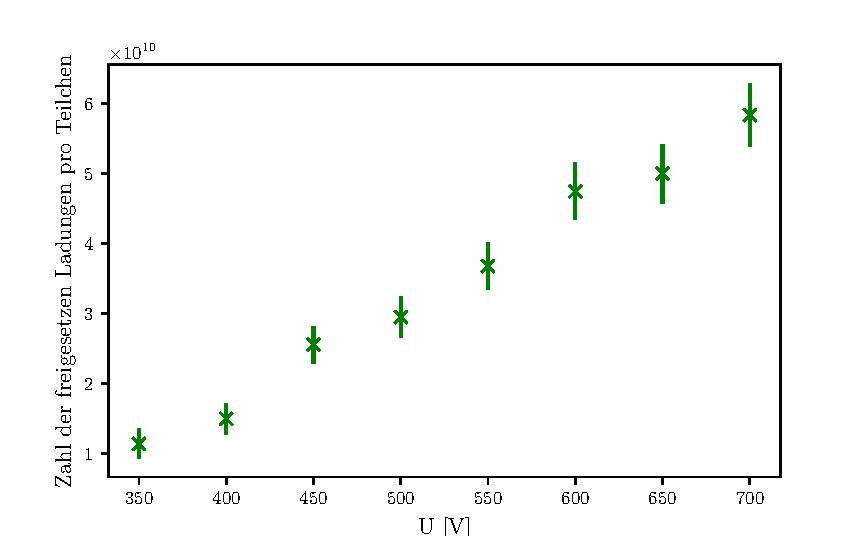
\includegraphics{plot1.pdf}
    \caption{Deltawerte}
    \label{fig:plot}
  \end{figure}

\subsection{Beugung am Gitter}
  Im letzen Teil des Versuchs soll nun die Wellenlänge des Lichtes bestimmt werden. Dazu 
  wird die Beugung an mehreren Gittern betrachtet. Die aufgenommenen Daten sind in Tabellen \ref{tab:gitter1},
  \ref{tab:gitter2} und \ref{tab:gitter3} zu finden.
  \begin{table}[H]
    \centering
    \caption{Gitter mit 600 Linien/mm}
    \begin{tabular}{c}
      \toprule
      Maximum 1\\
      \midrule
      23.2 \\
      22.7 \\
      \bottomrule
    \end{tabular}
    \label{tab:gitter1}
  \end{table}
  \begin{table}[H]
    \centering
    \caption{Gitter mit 300 Linien/mm}
    \begin{tabular}{c c}
      \toprule
      Maximum 1 & Maximum 2\\
      \midrule
      11   & 22.7 \\
      11.5 & 23.2 \\
      \bottomrule
    \end{tabular}
    \label{tab:gitter2}
  \end{table}
  \begin{table}[H]
    \centering
    \caption{Gitter mit 100 Linien/mm}
    \begin{tabular}{c c c c}
      \toprule
      Maximum 1 & Maximum 2 & Maximum 3 & Maximum 4\\
      \midrule
      4   & 7.7 & 11.5 & 15 \\
      3.6 & 7   & 11   & 15 \\
      \bottomrule
    \end{tabular}
    \label{tab:gitter3}
  \end{table}
  \noindent Anhand der Gleichung 
  \begin{equation*}
    \lambda = d \dfrac{\sin{\phi}}{k}
  \end{equation*}
  ist es nun möglich die Wellenlänge des Lichtes zu bestimmen. Die für die oben 
  gelisteten Daten berechneten Werte sind in Tabelle \ref{tab:wellen} aufgelistet.
  \begin{table}[H]
    \centering
    \caption{Wellenlänge, angegeben in m x $ 10^{7}$}
    \begin{tabular}{c c c c c}
      \toprule
      Gitterart & Maximum 1 & Maximum 2 & Maximum 3 & Maximum 4\\
      \midrule
      600&6.57   &&&\\
      &6.43&&&\\
      300&6.36& 6.43&& \\
      &6.65&6.57&&\\
      100&  6.98   &   6.7&  6.65&6.47 \\
      &6.27&6.09&6.36&6.47\\
      \bottomrule
    \end{tabular}
    \label{tab:wellen}
  \end{table}
  \noindent Der Mittelwert dieser Werte wurde mittels Numpy berechnet und liegt bei \\
  $\lambda=(6.5\pm0.06)\cdot 10^{-7}$